\section{Theorie}
\label{sec:Theorie}
Das Ziel des Versuchs ist es grundlegende Gesetzmäßigkeiten der Strahlenoptik in verschiedenen Versuchsteilen zu Untersuchen.
Licht besteht aus elektromagnetischer Strahlung. Die Ausbreitung von elektromagnetischen Wellen kann mit Hilfe der Maxwellschen Gleichungen beschrieben werden,
jedoch können für die Reflexion und Brechung an Grenzflächen die Regeln der Strahlenoptik verwendet werden. 
Die Ausbreitung der Wellen kann in der Strahlenoptik durch die Normalen der Wellenflächen, die senkrecht auf der Wellenfront stehen, beschrieben werden. 
Die Wellennormale wird in der Strahlenoptik Lichtstrahl genannt. Die Ausbreitungsgeschwindigkeit ist abhängig von dem Material in dem die Welle sich ausbreitet.
Der Lichtstrahl wird beim Übergang zwischen Material 1 mit dem Brechungsindex $n_1$ und Material 2 mit dem Brechungsindex $n_2$ gebrochen. Die Brechung wird durch die Beziehung
\begin{equation}
    \frac{\sin \alpha}{\sin \beta} = \frac{v_1}{v_2}= \frac{n_1}{n_2}
    \label{eqn:brech}
\end{equation}
beschrieben, wobei $v_k$ die Ausbreitungsgeschwindigkeit im jeweiligen Material, $\alpha$ der Einfallswinkel und $\beta$ der Brechungswinkel ist.
Ein Material ist optisch dichter, wenn die Ausbreitungsgeschwindigkeit der Welle in diesem Material größer ist. Ist sie kleiner wird das Material optisch dünner genannt.
In der Strahlenoptk breiten sich  die Lichtstrahlen in einem homogenen Material geradlinig aus und beeinflussen sich nicht gegenseitig.
Wird ein Lichtstrahl an einer Grenzfläche reflektiert, ergibt sich die Beziehung
\begin{equation}
    \alpha_1=\alpha_2
    \label{eqn:refl}
\end{equation}
für den Einfallswinkel $\alpha_1$ und den Reflexionswinkel $\alpha_2$.
Wird ein Lichtstrahl an einem Medium mit anderen Brechungsindex gebrochen, erfährt der Lichtstrahl an der Grenzfläche eine Richtungsänderung.
Nach dem Gesetz von Snellius ergibt sich
\begin{equation}
    n_1 \sin \alpha = n_2 \sin \beta
    \label{eqn:brechung}
\end{equation}
für die Beziehung der ein- und auslaufenden Welle.
\begin{figure}
    \centering
    \caption{Brechung an einem Medium mit verschiedenem Brechungsindex \cite{V400}}
    \label{fig:brech}
    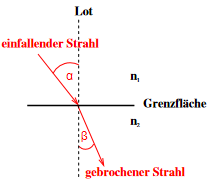
\includegraphics[width = 0.6 \textwidth]{pics/brechung.png}
\end{figure}
Dabei werden die Winkel $\alpha$ und $\beta$, wie in Abbildung \ref{fig:brech} zu sehen, abgelesen.
Das Verhältnis der Reflexion und der Brechung an der Grenzfläche zu einem anderen Medium ist Materialabhängig. Jedoch gilt immer $R+T=1$.
\\
Trifft Licht auf ein Hindernis, so kann beobachtet werden, dass sich das Licht im Schattenraum ausbreitet.
Für die Erklärung der Beugung reicht die Strahlenoptik nicht. Mit Hilfe der Wellenoptik kann dieses Phänomen erklärt werden.
Charakteristisch für eine elektromagnetische Welle ist die Frequenz $\nu$ bzw. die Wellenlänge $\lambda$ und die Ausbreitungsgeschwindigkeit $v$.
Überlagern sich zwei Wellen, so entspricht die resultierende Intensitätsverteilung der Summe der Einzelintensitäten. Da Licht aus zahlreichen Wellenzügen besteht, kommt es bei selber Frequent und fester Phasenbeziehung
zu einem Interfernzbild. Je nach Phasenbeziehung kommt es zu konstruktiver oder destruktiver Interferenz. Eine vollständige Auslöschung von zwei Wellen entsteht bei einem Gangunterschied von $\sfrac{d}{2}$.
In diesem Versuch wird die Beugung am Gitter untersucht. Es kommt zur Beugung, wenn ein Hindernis, dessen Abmessung klein im Vergleich zur Wellenlänge ist, im Weg der Wellenausbreitung ist.
Dabei kann die Ausbreitung der Welle mit dem Huygenschen Prinzip konstruiert werden, welches besagt, dass jeder Punkt einer Welle der Ausgangspunkt einer Elementarwelle gleicher Frequenz ist.
Ein einfaches Hindernis ist ein Spalt. Eine ebene Wellenfront die auf einen Spalt der Spaltbreite $a$ trifft, wird an allen Punkten in der Spaltöffnung gebeugt.
Befindet sich ein Schirm im Abstand $L$ vom Spalt, ergibt sich ein Interfernzmuster auf diesem. Dabei entstehen die Maxima an den Stellen, für die
\begin{equation}
    a \sin \alpha = k \lambda
    \label{eqn:einf}
\end{equation}
gilt. Dabei ist $\lambda$ die Wellenlänge des Lichtes, welches den Einfachspalt der Breite $a$ beleuchtet. Das k-te Intensitätsmaximum erscheint in einem Winkel von $\alpha$ relativ zur geradlinigen Ausbreitungsrichtung.
Ein Strichgitter besteht aus N-Einfachspalten gleicher Breite. Die Bedingungen für die Intensitätsmaxima k-ter Ordnung ergeben sich zu
\begin{equation}
    d \sin \alpha = k \lambda \, ,
    \label{eqn:gitter}
\end{equation}
wobei $d$ die Gitterkonstante ist.



